
\documentclass[draft]{agujournal2019}
\usepackage{url} %this package should fix any errors with URLs in refs.
\usepackage{lineno}
\usepackage[inline]{trackchanges} %for better track changes. finalnew option will compile document with changes incorporated.
\usepackage{soul}
\usepackage{pdflscape}
\linenumbers

\draftfalse


\journalname{Journal of Advances in Modeling Earth Systems (JAMES)}
\begin{document}
\title{The Community Land Model, version 5.1 \\ One-at-a-time Parameter Perturbation Ensemble}

\authors{D. Kennedy\affil{1} and ...}

\affiliation{1}{Climate and Global Dynamics Laboratory, NCAR, Boulder, CO, USA.}
\correspondingauthor{Daniel Kennedy}{djk2120@ucar.edu}

\begin{keypoints}
\item enter point 1 here
\end{keypoints}

\begin{abstract}
[ enter your Abstract here ]
\end{abstract}


\section{Introduction}
Water availability, land temperature extremes, fire risk, and crop productivity will all see impacts from climate change, and are among the many processes represented within land components of Earth System Models.
Understanding how these processes respond directly and indirectly to CO$_2$ concentrations, and how they themselves impact CO$_2$ concentrations, is a critical facet of climate change research.  
Our certainty in climate model projections varies by domain and generally decreases with extended time horizons \cite{koven2022}.
Centennial-scale estimates of the cumulative terrestrial carbon sink have been especially challenging, with high uncertainty persisting across model generations \cite{friedlingstein2014,arora2020}. 
A portion of this uncertainty is irreducible, inherent to the challenge of predicting vegetation dynamics in a novel climate \cite{lovenduski2017}.
But with the ever-increasing observational basis from remote sensing, meteorological stations, flux towers, and field campaigns, combined with increasingly comprehensive land surface modelling platforms, we might expect predictions to become more skillful across subsequent model generations.

While model inter-comparison projects have had tremendous utility, it can be difficult to interpret the differences between models, or even between subsequent versions of the same model, due to the multiplicity of structural and parametric variations \cite{mcneall2016}.
Within the model development process, there is a significant emphasis on hypothesis testing, substituting one parameterization at a time to understand the various consequences.
However, the complexity of land models has increased to the point where understanding the full span of model function has become challenging \cite{fisher2020}, and manual model calibration appears intractable \cite{dagon2020}.
Maintaining, improving, and interpreting complex land models benefits from thoughtful investment in software to automate and routinize important components of the development process, e.g. \citeA{collier2018}. 

One such fundamental model development step is parameter sensitivity testing and/or parameter optimization \cite{qian2018}.
Because parameter values are uncertain, evaluating the effect of parameter values on model output is critical to the model development process \cite{hourdin2017,balaji2022}.
When applied systematically, the result is a Parameter Perturbation Ensemble (PPE), alternatively termed a Perturbed Physics Ensemble.
PPEs have played an important role in assessing projection uncertainty in climate models \cite{murphy2004,sanderson2008,booth2012,hawkins2019,yamazaki2021,peatier2022,tett2022}.
PPEs also form a basis for automated model calibration through, for example, history matching \cite{williamson2013,williamson2017,hourdin2020,couvreux2021} or Bayesian uncertainty quantification \cite{cleary2021}.
Our goal in this project is to systematize parameter perturbation activity within our modeling framework, and develop the necessary tools and datasets to efficiently test parameter effects across the full suite of land model processes. 
In doing so, we have generated a large PPE, comprising thousands of parameter sensitivity tests.
In this paper we present that dataset, describe how it was produced, and survey some potential applications.

We are working with the Community Land Model (CLM), the land component of the Community Earth System Model, which is developed and maintained at the National Center for Atmospheric Research (NCAR).
This work follows up on \citeA{dagon2020}, which began the process of systematically varying CLM parameters in service of automated model calibration.
We extend that work by sampling a more exhaustive set of parameters across a broader range of land model processes.
A set of 193 parameters were varied across a range of climate scenarios.
This dataset has already demonstrated great utility for diagnosing parameter effects, while the software and modeling infrastructure has greatly our expanded our capability to generate insights about parameter effects and uncertainties within CLM.

\section{Experiment Description}
\label{methods}
\subsection{Model description}
\label{sect:md}
The Community Terrestrial Systems Model (CTSM) is developed by the CESM Land Model Working Group and maintained at the National Center for Atmospheric Research (NCAR). This experiment utilizes the Community Land Model configuration of CTSM, version 5.1 (CLM5.1). The model source code and documentation are available online (\url{https://github.com/ESCOMP/CTSM}), as is a full model description \cite{lawrence2019}.

Relative to CLM5.0, version 5.1 includes minor bug fixes, parameter adjustments, and the implementation of biomass heat storage \cite{swenson2019}. The PPE experiment required additional code modifications to systematically vary the full suite of model parameters. The model code for this experiment is contained in a development tag (\url{https://github.com/ESCOMP/CTSM/tree/branch_tags/PPE.n11_ctsm5.1.dev030}). We utilized the biogeochemistry version of CLM in land-only mode, with the crop model turned off. The component set longname is: \\ \texttt{2000\_DATM\%GSWP3v1\_CLM51\%BGC\_SICE\_SOCN\_SROF\_SGLC\_SWAV\_SIAC\_SESP}

\subsection{Model spin-up}
\label{sect:mcn}
Model spin-up for the equilibration of carbon and nitrogen pools within biogeochemistry-enabled land models can consume up to 98\% of computational time needed for a simulation \cite{sun2023}. Depending on the evaluation criteria and model configuration, CLM5 requires between 800 and 2000 years (or more) to reach steady-state conditions \cite{lawrence2019}. In the absence of equilibrium, the drift towards steady state can obscure important model dynamics or features. For this reason, each member of the PPE has a unique steady state and thus requires an independent spin-up.

To manage computational cost we leveraged the Matrix-CN spin-up mode recently implemented within CLM \cite{lu2020}. This new module utilizes a linearized simplification of CLM's biogeochemistry to significantly reduce spin-up time. Our spin-up protocol featured 20 years in accelerated decomposition mode, followed by 80 years of Matrix-CN, followed by 40 years of `normal' mode, cycling over a ten-year forcing dataset (described below). This protocol was designed to achieve sufficiently equilibrated model states, while minimizing computational time. This spin-up methodology did not always reach full equilibration of deep soil carbon (beyond 1 meter depth). Certain inferences about deep soil carbon are therefore subject to uncertainty due to spin-up concerns.

\subsection{Sparsegrid}
\label{sect:sg}
Another control on model cost is resolution. Most CLM simulations utilize nominal 1$^\circ$ resolution, which requires over 20,000 land grid cells. In order to manage computational cost, parameter perturbation experiments often use lower resolution, such as 4$^\circ$x5$^\circ$ \cite{dagon2020}. Here, we use a clustering algorithm to achieve an alternative low resolution configuration.

Multivariate spatio-temporal clustering (MVSC) has been utilized to extract patterns of climatological significance from climate model output \cite{hoffman2005} and applied to design a representativeness-based sampling network \cite{hoffman2013}. Instead of lowering resolution by coarsening a rectilinear grid, we used MVSC to strategically remove redundant grid cells, leaving only 400 grid cells that efficiently sample important model dynamics.

We used k-means clustering to identify groups of grid cells with similar dynamics based on a 2$^\circ$ transient simulation (1850-2014) using the CLM-PPE codebase. We selected one representative grid cell from each cluster to stand in for the entire cluster. The representative grid cell is whichever is located nearest the cluster centroid in climate space. The set of representative grid cells comprise a `sparsegrid', which are used in lieu of a `coarse' grid. To recompose mapped output and compute global means, the output from the representative grid cell is substituted for all members of the cluster cohort.

Clustering was based on a subset of 18 meaningful CLM variables (Table \ref{tab:sg}). The clustering algorithm analyzed 12 observations of each variable per grid cell, namely the mean and interannual variability computed for six 30-year climatology windows (1865-1894, 1895-1924, ... , 1985-2014). Clusters were delineated to equalize the multi-dimensional variance across the user-specified number of groups, $k$. We tested 15 values of $k$, ranging from 10 to 800. Based on ILAMB2.5 benchmarking \cite{collier2018} against the full grid output, we opted for a 400-cluster sparsegrid, to balance computational cost against model fidelity (Supp Figure \ref{supp:ilamb}). Because our emphasis is on vegetated regions, we masked out Antarctica within the clustering algorithm, whereby we do not provide any output below 60$^\circ$S.

\begin{table}[h]
\caption{Clustering inputs categorized into three groups, with the CLM variable name in parentheses}
\centering
\begin{tabular}{l c c c c}
 \hline
 Climate forcing variables & Ecosystem state variables &Ecosystem flux variables \\
 \hline
 2m air temperature (TSA) & Leaf area index (TLAI) & Gross primary production (GPP) \\
Atmospheric rain (RAIN) & Ecosystem carbon (TOTECOSYSC) &Heterotrophic respiration (HR) \\
Atmospheric snow (SNOW) &  Ecosystem nitrogen (TOTECOSYSN) &Autotrophic respiration (AR) \\
2m specific humidity (Q2M) & Soil ice (TOTSOILICE) &Net biome production (NBP) \\
Solar radiation (FSDS) & Soil liquid water (TOTSOILLIQ) & Total liquid runoff (QRUNOFF) \\
& Snow cover fraction (FSNO) & Sensible heat  (FSH) \\
&&Latent heat (EFLX\_LH\_TOT ) \\
 \hline
 \end{tabular}
 \label{tab:sg}
 \end{table}


\subsection{Experimental Design}
In the preparation for this experiment, 188 CLM-BGC parameters were identified. We decided to vary each parameter independently, to a low and high values. To define parameter ranges we created an online spreadsheet and solicited domain-area experts to provide a minimum and maximum value for each parameter. In some cases literature values were directly utilized, but in the majority of cases, expert judgment was used. The spreadsheet, with literature references and parameter descriptions is available online and in appendix zqz. In some cases parameters could not be perturbed independently, because they are required to sum to 1. In the case of nitrogen fixation costs, we opted to perturbed the parameters independently, but also as a group (`KCN'), to enforce nitrogen limitation in lieu of switching from one uptake pathway to another.

Each simulation ran for 150 years, with the first 140 for spin-up, followed by a 10-year period for analysis. We opted for six different forcing scenarios to understand the intersection of parameter effects and climate change (Table \ref{tab:exps}). The GSWP3v1 reanalysis product (\url{http://hydro.iis.u-tokyo.ac.jp/GSWP3/}) served as our atmospheric forcing, and is the default forcing data for CLM5 \cite{lawrence2019}. We applied climate and CO$_2$ anomalies independently, in order to disentangle their effects on parameter rankings. Future and pre-industrial climate forcing datasets were prepared by adding GSWP3v1 anomalies from 2005-2014 to the corresponding mean climate change signal (see Table \ref{tab:exps}). We inferred the mean climate change signal using the CESM2 large ensemble experiment \cite{rodgers2021}, computed as the average of the difference between the period of interest and present day for the six atmospheric forcing variables.

\label{sect:exps}
 \begin{table}[h]
 \caption{Forcing Scenarios}
 \centering
 \begin{tabular}{l c c c c}
 \hline
  Name  & Meteorology & CO$_2$ (ppmv) & N addition & Description \\
 \hline
   CTL2010  & 2005-2014 & 367 & - & control experiment\\
   C285        & 2005-2014 & 285 & - & low CO$_2$ \\
   C867        & 2005-2014 & 867 & - & high CO$_2$ \\
   AF1855    & 1851-1860 & 367 & - & pre-industrial climate \\
   AF2095    & 2091-2100 & 367 & - & late century climate (SSP3-7.0) \\
   NDEP      & 2005-2014 & 367 & 5g/m$^2$ & enhanced nitrogen deposition \\
 \hline
 \end{tabular}
 \label{tab:exps}
 \end{table}

\subsection{Parameters} 
\begin{landscape}
 \begin{table}[h]
 \caption{Some key parameters}
 \centering
 \begin{tabular}{l l c}
 \hline
  Parameter  & Description & Model Domain \\
 \hline
d\_max & Dry surface layer (DSL) parameter & Sensible, latent heat and momentum fluxes \\
frac\_sat\_soil\_dsl\_init & Fraction of saturated soil at which DSL initiates & Sensible, latent heat and momentum fluxes \\
fff & Decay factor for fractional saturated area & Hydrology \\
liq\_canopy\_storage\_scalar & Canopy-storage-of-liquid-water parameter & Hydrology \\
maximum\_leaf\_wetted\_fraction & Maximum leaf wetted fraction & Hydrology \\
medlynintercept & Medlyn intercept of conductance-photosynthesis relationship & Stomatal resistance and photosynthesis \\
medlynslope & Medlyn slope of conductance-photosynthesis relationship & Stomatal resistance and photosynthesis \\
tpu25ratio & Ratio of tpu25top to vcmax25top & Stomatal resistance and photosynthesis \\
jmaxb0 & Baseline proportion of nitrogen allocated for electron transport & Photosynthetic capacity (LUNA) \\
jmaxb1 & Response of electron transport rate to light & Photosynthetic capacity (LUNA) \\
slatop & Specific leaf area at top of canopy & Photosynthetic capacity (LUNA) \\
wc2wjb0 & Baseline ratio of wc:wj & Photosynthetic capacity (LUNA) \\
kmax & Plant segment max conductance & Plant hydraulics \\
krmax & Root segment max conductance & Plant hydraulics \\
psi50 & Water potential at 50\% loss of conductance & Plant hydraulics \\
nstem & Stem number & Biomass heat storage \\
lmr\_intercept\_atkin & Intercept in the calculation of leaf maintenance respiration& Plant respiration \\
froot\_leaf & Allocation parameter: new fine root C per new leaf C & Carbon and nitrogen allocation \\
leafcn & Leaf C:N & Carbon and nitrogen allocation \\
leaf\_long & Leaf longevity & Vegetation phenology and turnover \\
cpha & Activation energy for cp & Acclimation parameters \\
jmaxhd & Deactivation energy for jmax & Acclimation parameters \\
kcha & Activation energy for kc & Acclimation parameters \\
lmrha & Activation energy for lmr & Acclimation parameters \\
lmrhd & Deactivation energy for lmr & Acclimation parameters \\
tpuha & Activation energy for tpu & Acclimation parameters \\
tpuse\_sf & Scale factor for tpu entropy term & Acclimation parameters \\
vcmaxha & Activation energy for vcmax & Acclimation parameters \\
vcmaxhd & Deactivation energy for vcmax & Acclimation parameters \\
 \hline
 \end{tabular}
 \end{table}
\end{landscape}


\subsection{Analyses}

Biome analysis

\section{Results}

A total of 193 parameters were targeted for sensitivity testing across a wide variety of CLM subcomponents (Figure \ref{fig:params}). In some cases new parameters were introduced to allow perturbation of important processes. For example a sand perturbation factor ($sand\_pf$) was introduced in order to perturb the percent sand in the soil column without creating a new surface dataset.  A spreadsheet detailing all of the parameters, and their ranges, is provided in the supplementary material and available online (zqz link).

\begin{figure}[h]
\centering
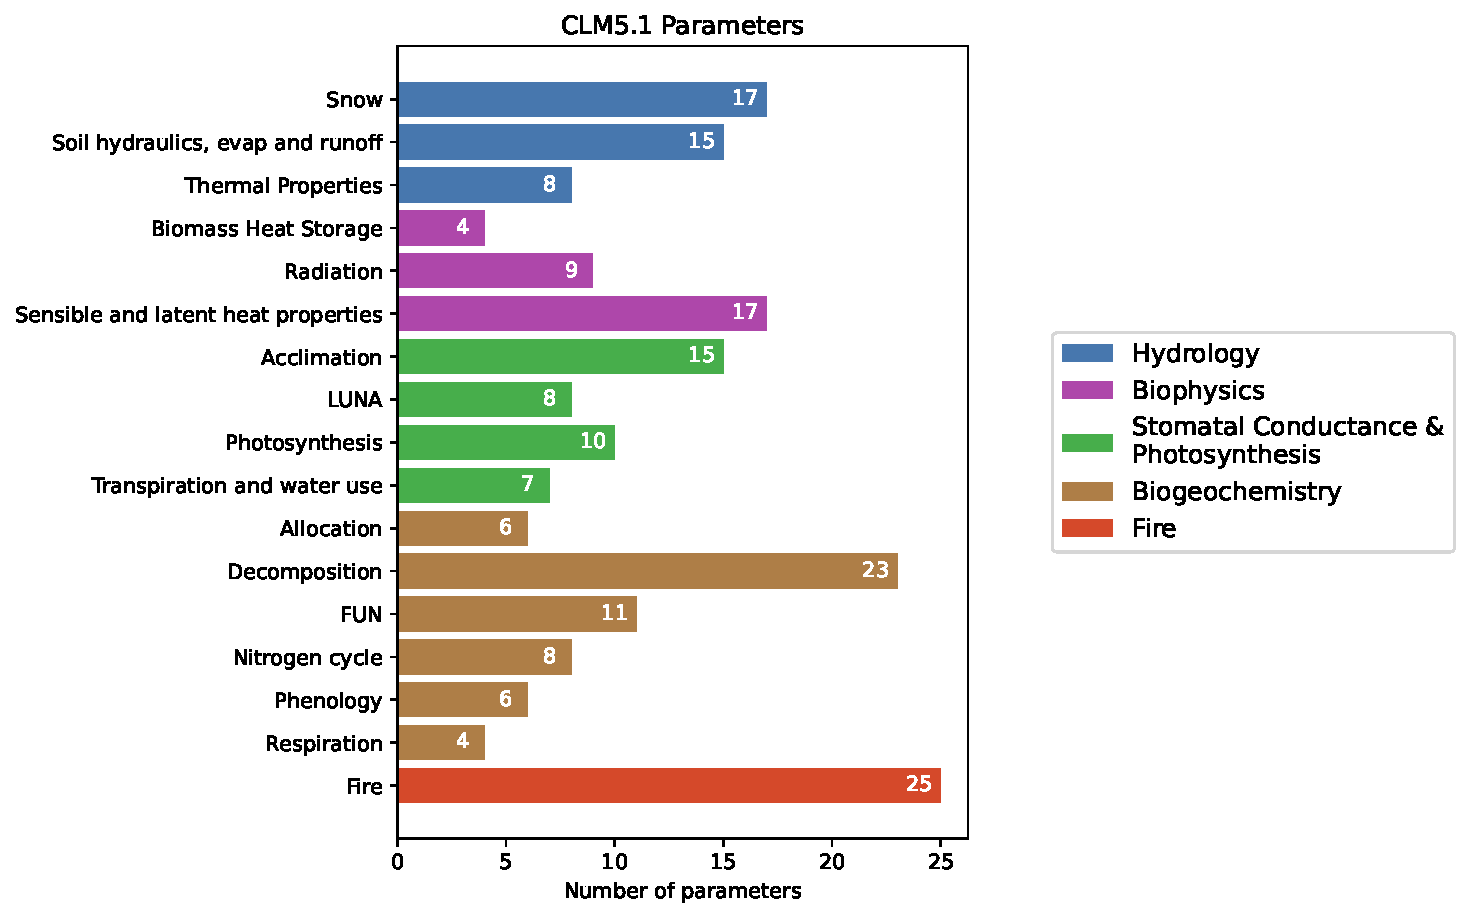
\includegraphics[width=\textwidth]{../figs/bar.pdf}
\caption{193 parameters were perturbed across the various domains of the land model.}
\label{fig:params}
\end{figure}

A major goal of this project was to develop a fast configuration of CLM5-BGC that would allow for a large number of simulations given the available computational resources.
Combining the CN-Matrix spinup approach with our sparsegrid formulation (see Section \ref{sect:sg} for details) yielded a configuration approximately 500 times faster than the 1-degree configuration most often used for CLM simulations (Figure \ref{fig:sims}).
There are 22648, 5666, and 1764 land grid cells in standard 1$^{\circ}$, 2$^{\circ}$, and 4$^{\circ}$x5$^{\circ}$ CLM simulations, respectively, as compared to just 400 grid cells in the sparsegrid.
Likewise, whereas previous spin-up methodologies required 1500 years or longer to satisfy equilibrium criteria, the CN-matrix approach yielded satisfactory spin-up for our experiment within 140 years.


\begin{figure}[h]
\centering
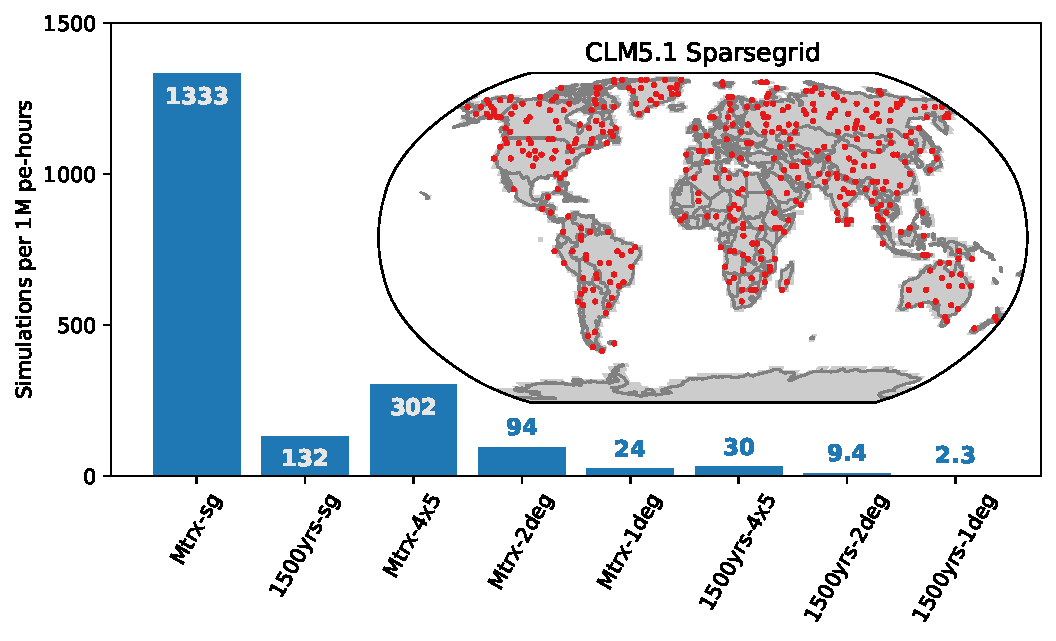
\includegraphics[width=30pc]{../figs/sims.pdf}
\caption{The approximate number of simulations afforded by 1 million core-hours for a range of CLM configurations. Configurations are labeled according to spin-up procedure (CN-matrix or the standard 1500-year spinup) and horizontal resolution (`sg' signifies sparsegrid). The inset map shows the locations of the 400 sparse grid cells. See Section \ref{methods} for spin-up and sparsegrid details.}
\label{fig:sims}
\end{figure}


Choosing the number of clusters to generate the sparsegrid involved balancing the computational savings against representational fidelity. Generally the more clusters, the 
better the approximation of output from the full grid can be achieved with the sparsegrid (Figure \ref{fig:sg}). Accuracy of global photosynthesis could be achieved with a relatively small number of clusters, with R$_2>$0.95 achieved with only 200 clusters, and RMSE$<$1PgC requiring approximately 700 clusters (Supp Figure zqz). We chose 400 clusters, based on ILAMB scores of a wide variety of output variables (Supp Figure \ref{supp:ilamb})
\begin{figure}[h]
\centering
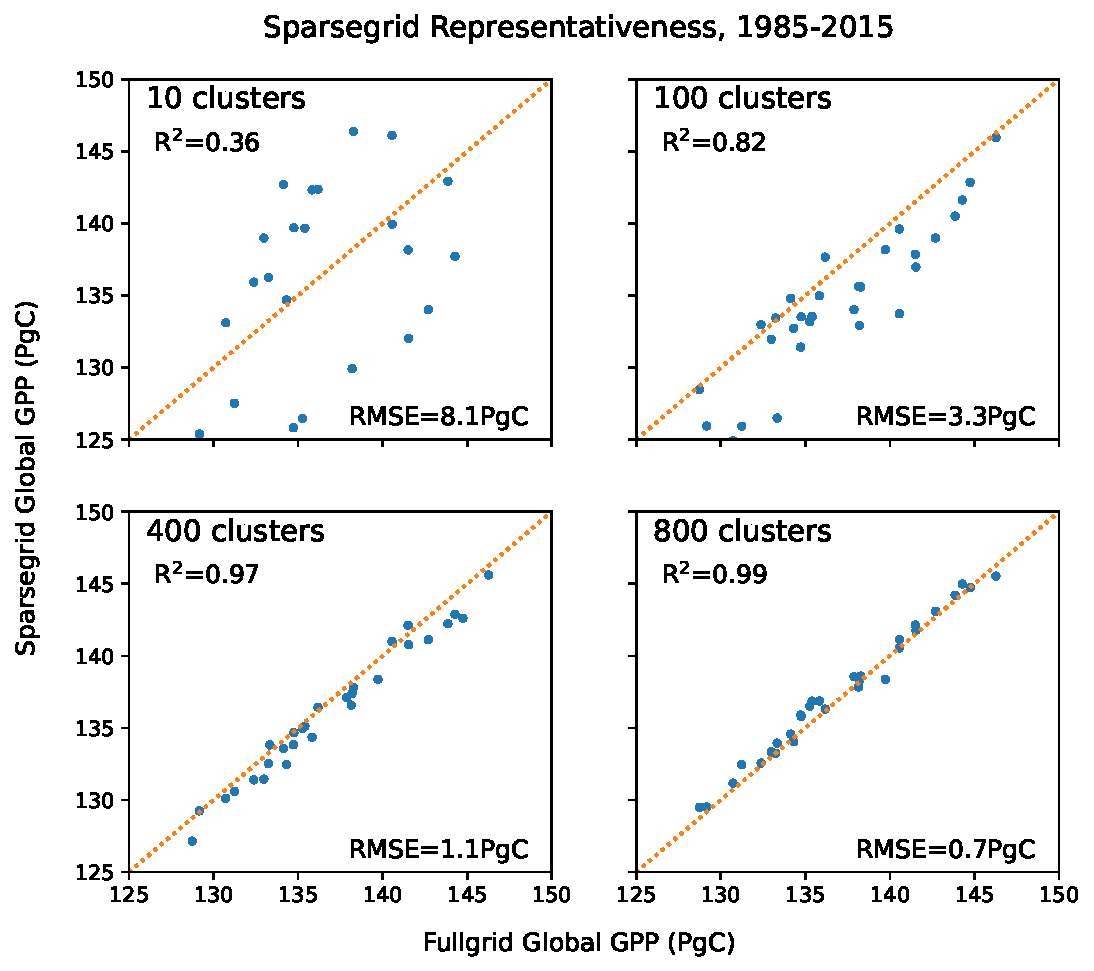
\includegraphics[width=25pc]{../figs/sparsegrid_gpp.pdf}
\caption{Sparsegrid vs fullgrid (2$^{\circ}$ resolution) global annual gross primary production (GPP) across the last forty years of a transient CLM5.1 simulation. We opted for 400 clusters to balance computational cost against representativeness.}
\label{fig:sg}
\end{figure}

Most of the parameter perturbations had a relatively small impact on any given output variable. For example, the distributions of GPP and NEP are concentrated around the default simulation with long tails, indicating that only a small proportion of parameters have large effects (Figure \ref{fig:violins}). One perturbation, reducing the heat capacity of sand by 20\%, proved destructive in the future climate scenario, resulting in inhospitably hot soil conditions and widespread plant death. This simulation is likely unrealistic, indicating that the perturbation range was too large, but possibly also that the model struggles to acclimate to warmer soils. This represents one of the valuable outcomes of an extensive PPE, exposing unexpected model behavior, which may belie brittle parameterizations or bugs.

\begin{figure}[h]
\centering
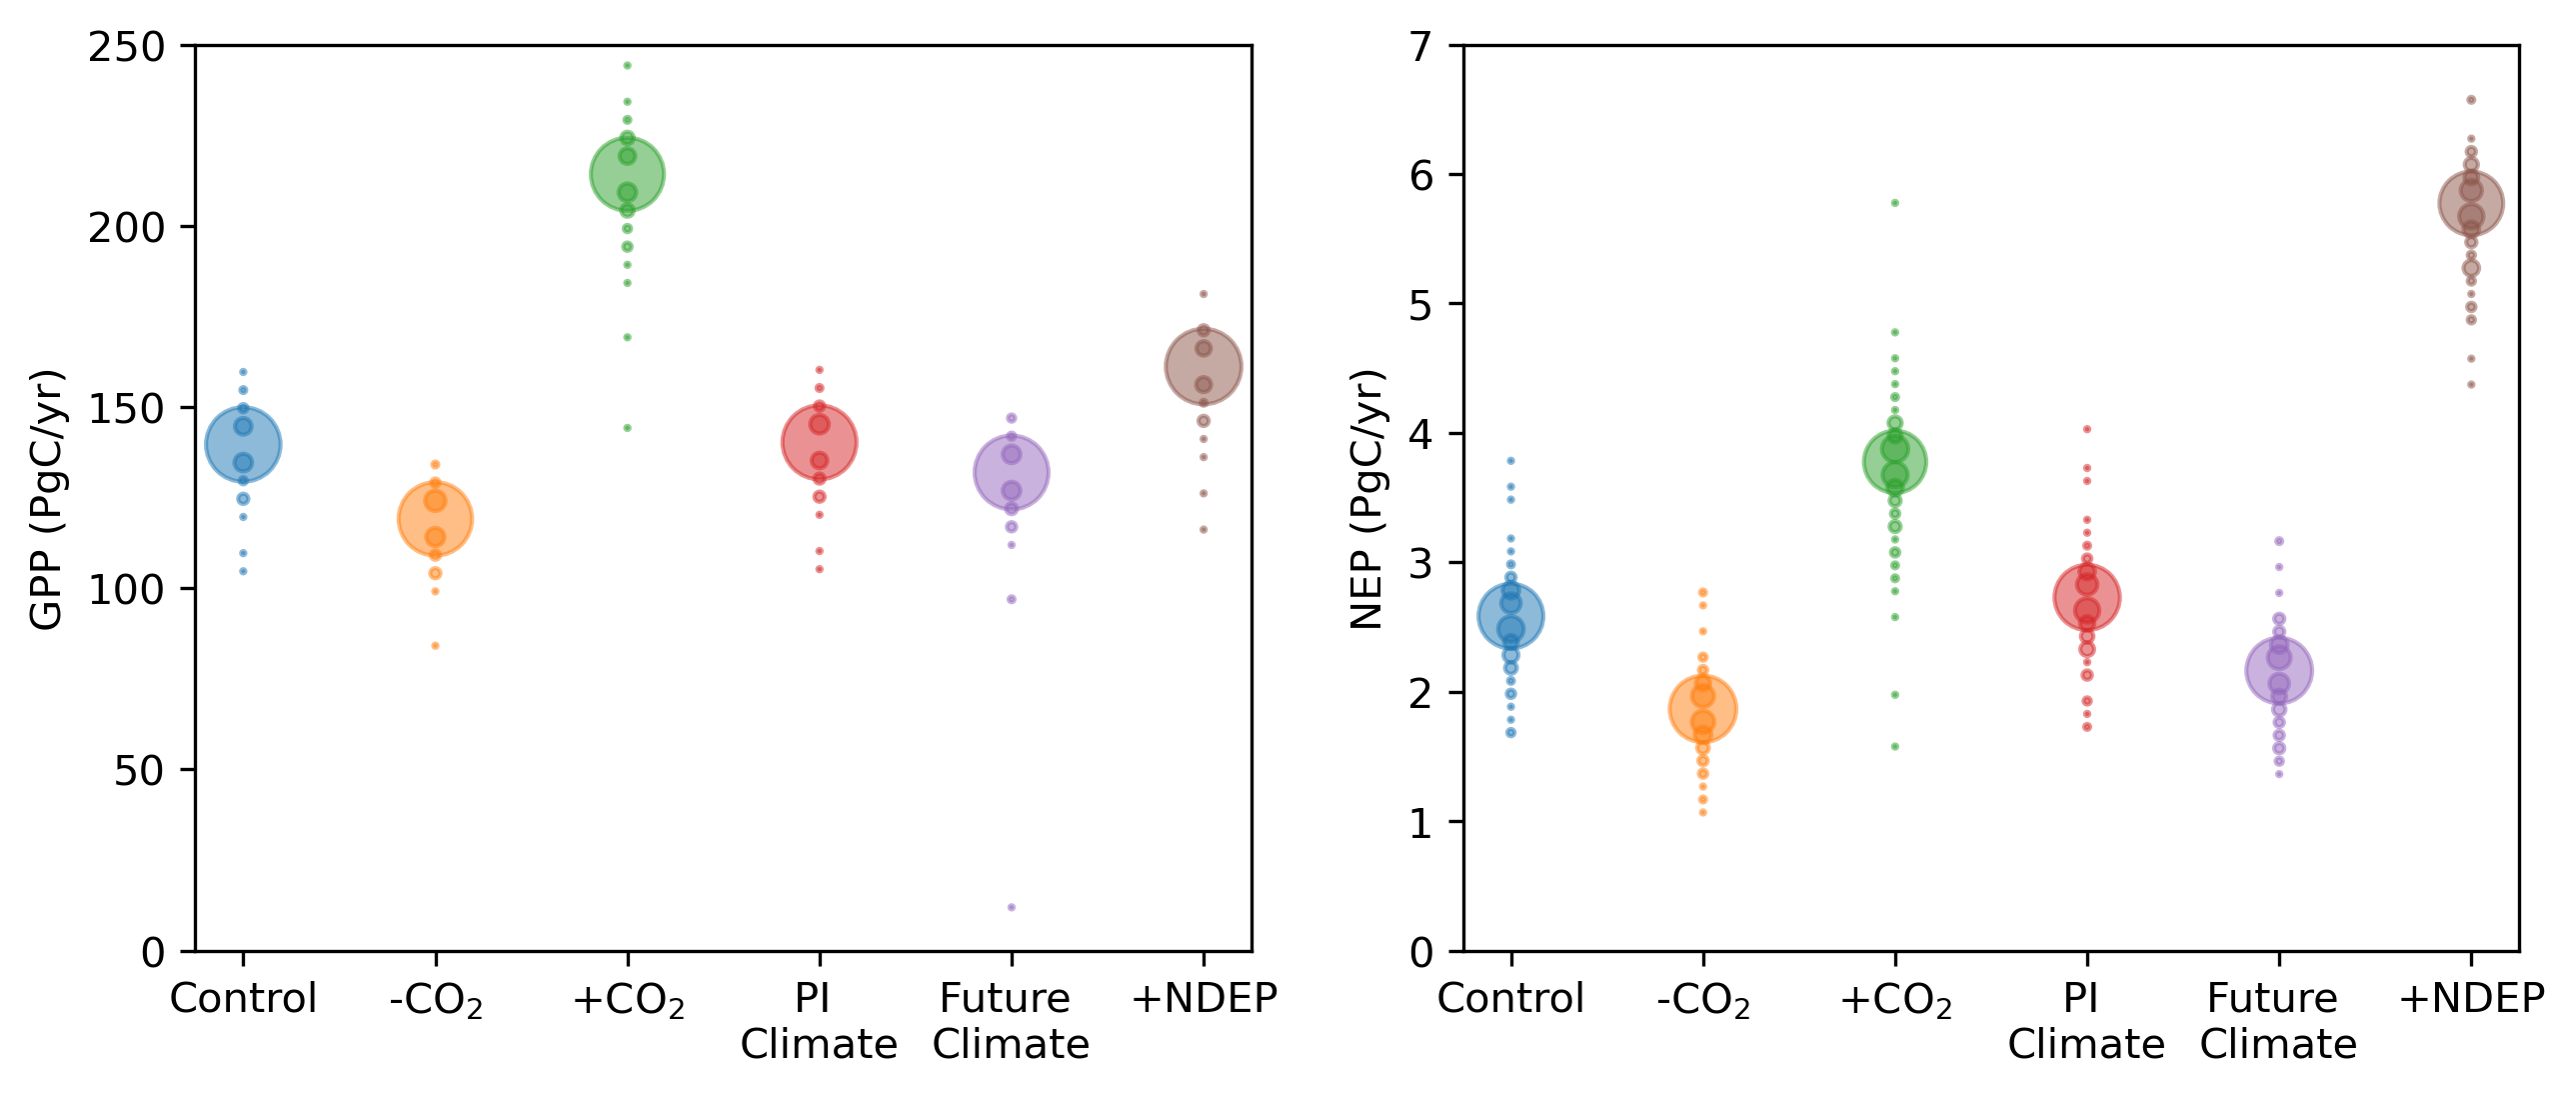
\includegraphics[width=\textwidth]{../figs/violins.png}
\caption{Global annual gross primary production (GPP) and net ecosystem production (NEP) across the PPE within each of our six forcing scenarios. Markers are drawn for 10 and 0.28 PgC bins for GPP and NEP, respectively. The marker area is proportional to the number of simulations falling in that bin. In each case the ellipse is centered about the default simulation.}
\label{fig:violins}
\end{figure}

\begin{figure}[h]
\centering
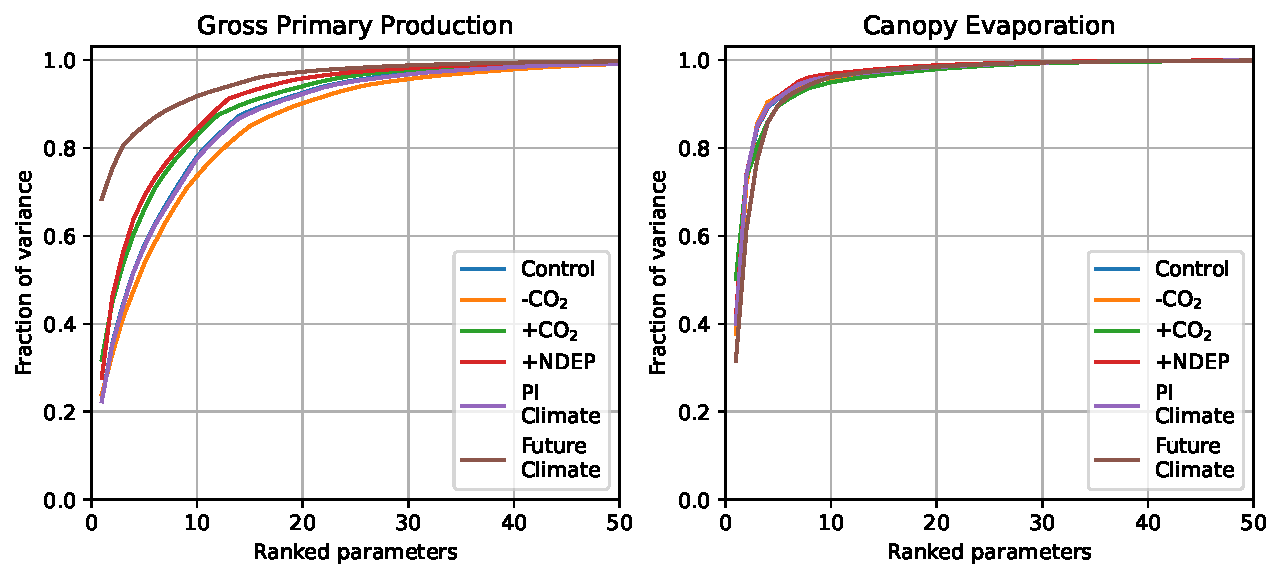
\includegraphics[width=\textwidth]{../figs/variance.pdf}
\caption{needs caption}
\label{fig:violins}
\end{figure}

Repeating our perturbations across the six forcing scenarios ensures that we can identify important parameters not just under present-day conditions, but also in the future. In the case of evaporation (ET), the parameters that control the increase in ET due to warming tend to be different from the parameters that control present-day ET (Figure \ref{fig:et}). 
ET response can differ significantly from the default case (i.e. stray from the orange line), even when ET is near the default under present-day conditions (i.e. within the shaded region).
All of the new parameters that appear in the ET response parameter rankings govern plant acclimation to temperature. 
These parameters, while not especially influential on present-day ET, are among the most important in governing the trend in ET going forward.

\begin{figure}[h]
\centering
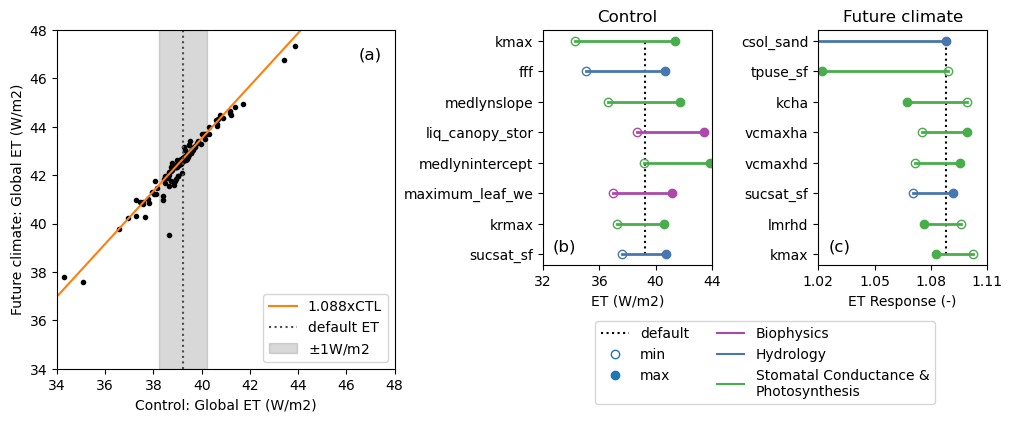
\includegraphics[width=\textwidth]{../figs/ET_response.png}
\caption{(a) Global annual average evapotranspiration (ET) in the warm forcing scenario vs. our control experiment. The shading spans the default ET in the control experiment, $\pm$1 W/m2. The response of ET to future climate with default parameters is +8.8\%. The orange line shows the expected future ET should the model conform to the default ET response. 
(b) The top 8 parameters governing global ET in the control experiment.
(c) The top 8 parameters governing ET response to future climate, i.e. the ratio of future ET to control ET.
Parameters governing the change in ET expected in the future tend to differ from the parameters controlling present-day ET.}
\label{fig:et}
\end{figure}

The PPE is likewise useful for determining which parameters influence which model processes and where. For example the parameters controlling leaf area index vary significantly by biome (Figure \ref{fig:lai}). Plant hydraulics parameters were the most important in the tropical rain forest, photosynthetic capacity in the boreal forest, and runoff and soil evaporation in the temperate grassland/desert biome. The most influential parameters globally include parameters from each of these three biomes. We have similar plots delineated by plant functional type, and for many other output variables in our extended diagnostics set (\url{https://webext.cgd.ucar.edu/I2000/PPEn11_OAAT}). 

\begin{figure}[h]
\centering
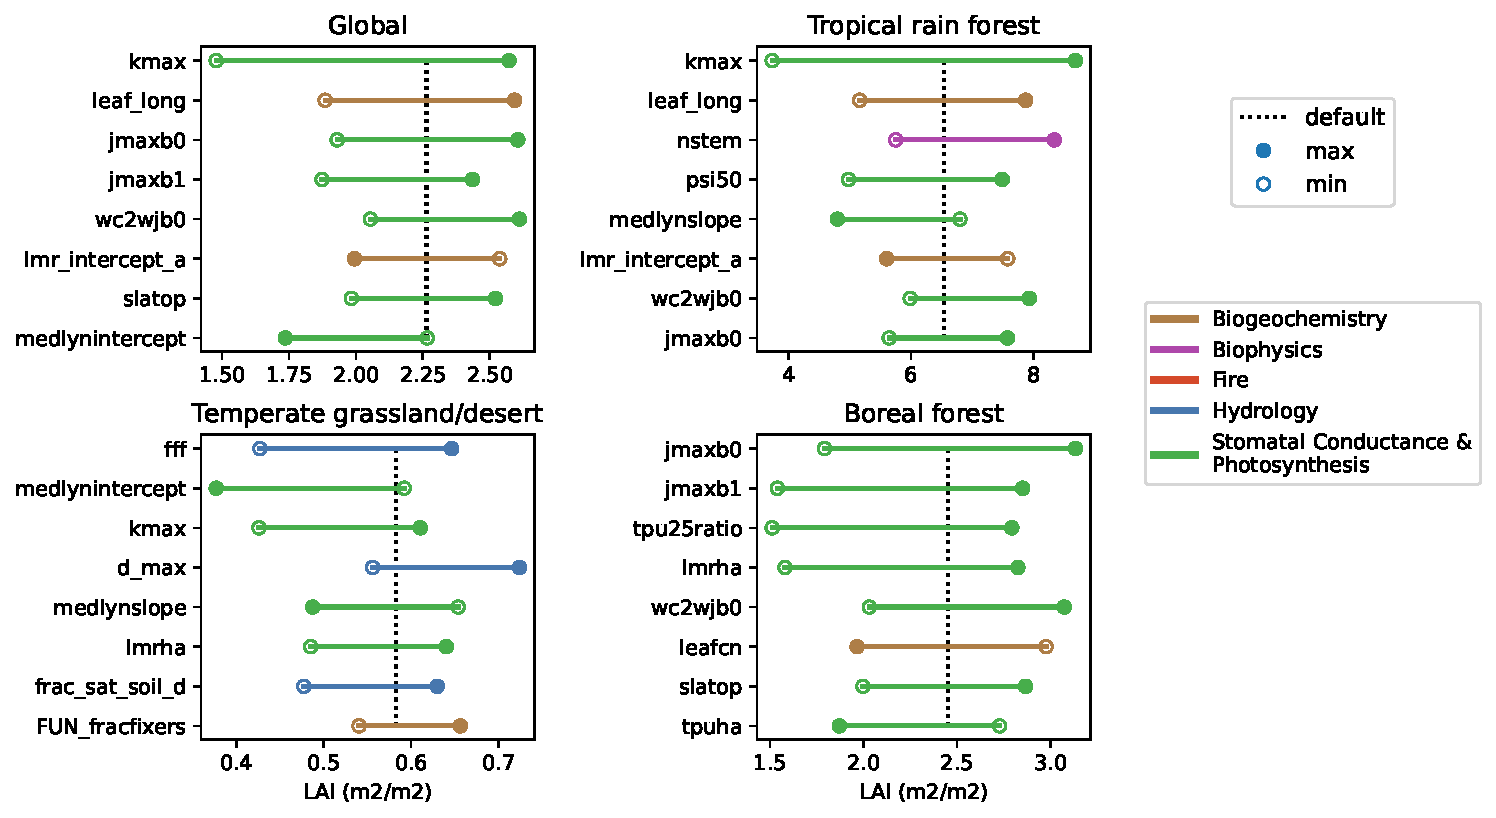
\includegraphics[width=\textwidth]{../figs/lai_biome.pdf}
\caption{The eight most influential parameters on leaf area index within the control ensemble, globally and within three biomes.}
\label{fig:lai}
\end{figure}



The volume of data generated by a large PPE can be overwhelming - our full dataset exceeds 2TB.  Our diagnostics package, which operates on only a subset of output variables, generated 1720 figures (\url{https://webext.cgd.ucar.edu/I2000/PPEn11_OAAT}). In many cases we have found it easier to utilize interactive plotting utilities to toggle through the various parameters, output variables, and forcing scenarios (Figure \ref{fig:panel}). Interactive widgets are relatively easy to generate within a data analysis session, but more difficult to host online, hence the screenshot.

\begin{figure}[h]
\centering
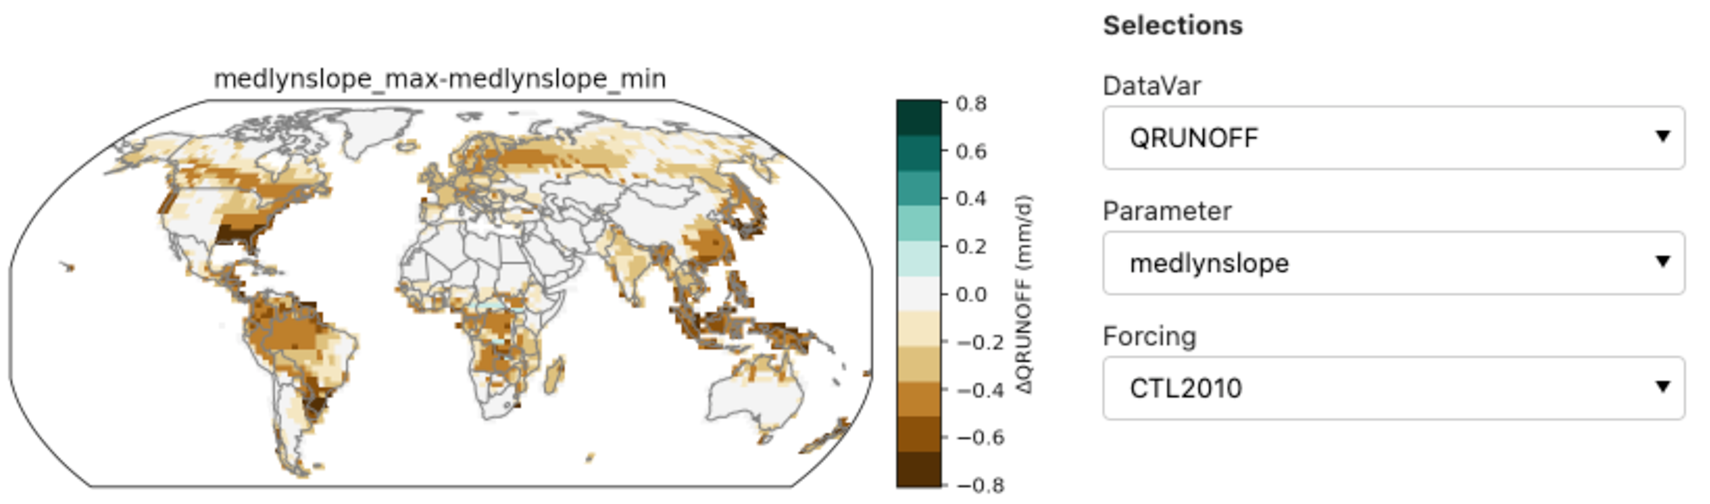
\includegraphics[width=\textwidth]{../figs/deltmap_panel.pdf}
\caption{Screenshot of interactive diagnostic for exploring maps of parameter effects. In this case, the effect of medlynslope on runoff within the control ensemble. Increasing medlynslope tends to reduce runoff, but only in regions with sufficient vegetation activity.}
\label{fig:panel}
\end{figure}

\section{Discussion}

In this project, we have identified and perturbed 188 CLM parameters to create a large one-at-a-time parameter perturbation ensemble. This ensemble is useful for understanding parametric controls on CLM processes and has already been leveraged as a starting point for parameter optimization efforts. We made significant investments in software infrastructure to enable this experiment and reduce the burden of generating future PPEs.

There were several barriers to perturbing the full set of CLM5-BGC parameters. Firstly, many parameters had not been officially identified as such. In such cases, we identified hard-coded values, established an appropriate parameter name, and extracted that parameter to the CLM parameter file for easier manipulation. In the end, we perturbed 188 parameters across a variety of CLM processes (Figure \ref{fig:params}). The second challenge involved defining a perturbation range for each parameter. We solicited expert judgment to set a minimum and maximum reasonable value for each parameter. In some cases, literature values were explicitly used (e.g. medlynslope), but the most common range was $\pm20\%$. The third challenge involved computational cost.

Running CLM-BGC with standard spin-up at 1$^\circ$ resolution, which is the most common configuration, would be prohibitively expensive, yielding only 2.3 simulations per million core-hours (for reference the CLM annual computing allocation is ~40 million core-hours). We sought a 2400-simulation ensemble, requiring a much faster model configuration. We sped up the model approximately 500x (Figure \ref{fig:sims}) by strategically reducing the number of model grid cells and by leveraging a linearized spin-up solver (see Sections \ref{sect:mcn} and \ref{sect:sg} for details). We found that most of the important model dynamics could be effectively resolved using only 400 grid cells and a 140-year spin-up sequence (Figure \ref{fig:sg}, Supp Figures \ref{supp:ilamb} and zqz spinup figure).

We found that parameter effects could be quite large, in some cases exceeding the effects of our various forcing scenarios (Figure \ref{fig:violins}). That being said, the majority of parameter perturbations had very small effect, leading to output distributions strongly concentrated around the default simulation with long tails representing a small subset of parameters. In the case of gross primary production, only xx parameters had a parameter effect of more than 2\% under the control forcing scenario (Supp Figure \ref{supp:gpp}). As such, we would expect that the dimensionality of the effective parameter space for any given process would be significantly smaller than implied by the 188 parameters.

We opted for six forcing scenarios to identify parameter effects not just in present-day but in response to pre-industrial or future climate conditions. The parameters that were most influential under present-day conditions did not necessarily match the set of parameters controlling the response to future forcing (Figure \ref{fig:et}). We found that many acclimation parameters, which were not as important for determining present-day evapotranspiration (ET), were among the most influential on the response of ET to future climate. Similarly, the parameters controlling leaf area index varied significantly depending on biome (Figure \ref{fig:lai}).

A one-at-a-time PPE cannot capture parameter interactions, and our min/max sampling protocol precludes diagnosing non-linearities. As such, this dataset will be insufficient for most calibration activities or for estimating overall parametric uncertainty. The advantage of our dataset is that we can diagnose parameter effects without the uncertainty of an approximating emulator or regression model. As such, it is easy to diagnose which parameters are most influential on a given process, which has been leveraged for parameter filtering. We have published a large set of ensemble diagnostic plots online, which serves as a valuable enhancement to our model technical documentation. Now in addition to seeing the definition of a given parameter, and the relevant equations, a model user can see the magnitude and spatial patterns of its effects (e.g. Figure \ref{fig:panel}).

We have already begun a follow-on experiment that perturbs a subset of parameters with the Latin hypercube sampling strategy to work towards calibrating leaf area index. By investing in the infrastructure underlying this first experiment, all of our subsequent experiments have required much less time and effort. We expect to continue to extend our efforts in this domain, as well as repeat these types of experiments with subsequent model releases.

\section{Conclusion}
\section*{Open Research Section}
This section MUST contain a statement that describes where the data supporting the conclusions can be obtained. Data cannot be listed as ''Available from authors'' or stored solely in supporting information. Citations to archived data should be included in your reference list. Wiley will publish it as a separate section on the paper’s page. Examples and complete information are here:
https://www.agu.org/Publish with AGU/Publish/Author Resources/Data for Authors


\acknowledgments
Enter acknowledgments here. This section is to acknowledge funding, thank colleagues, enter any secondary affiliations, and so on.




\bibliography{refs}

\appendix
\section{Supplementary Figures}


\begin{figure}[h]
\centering
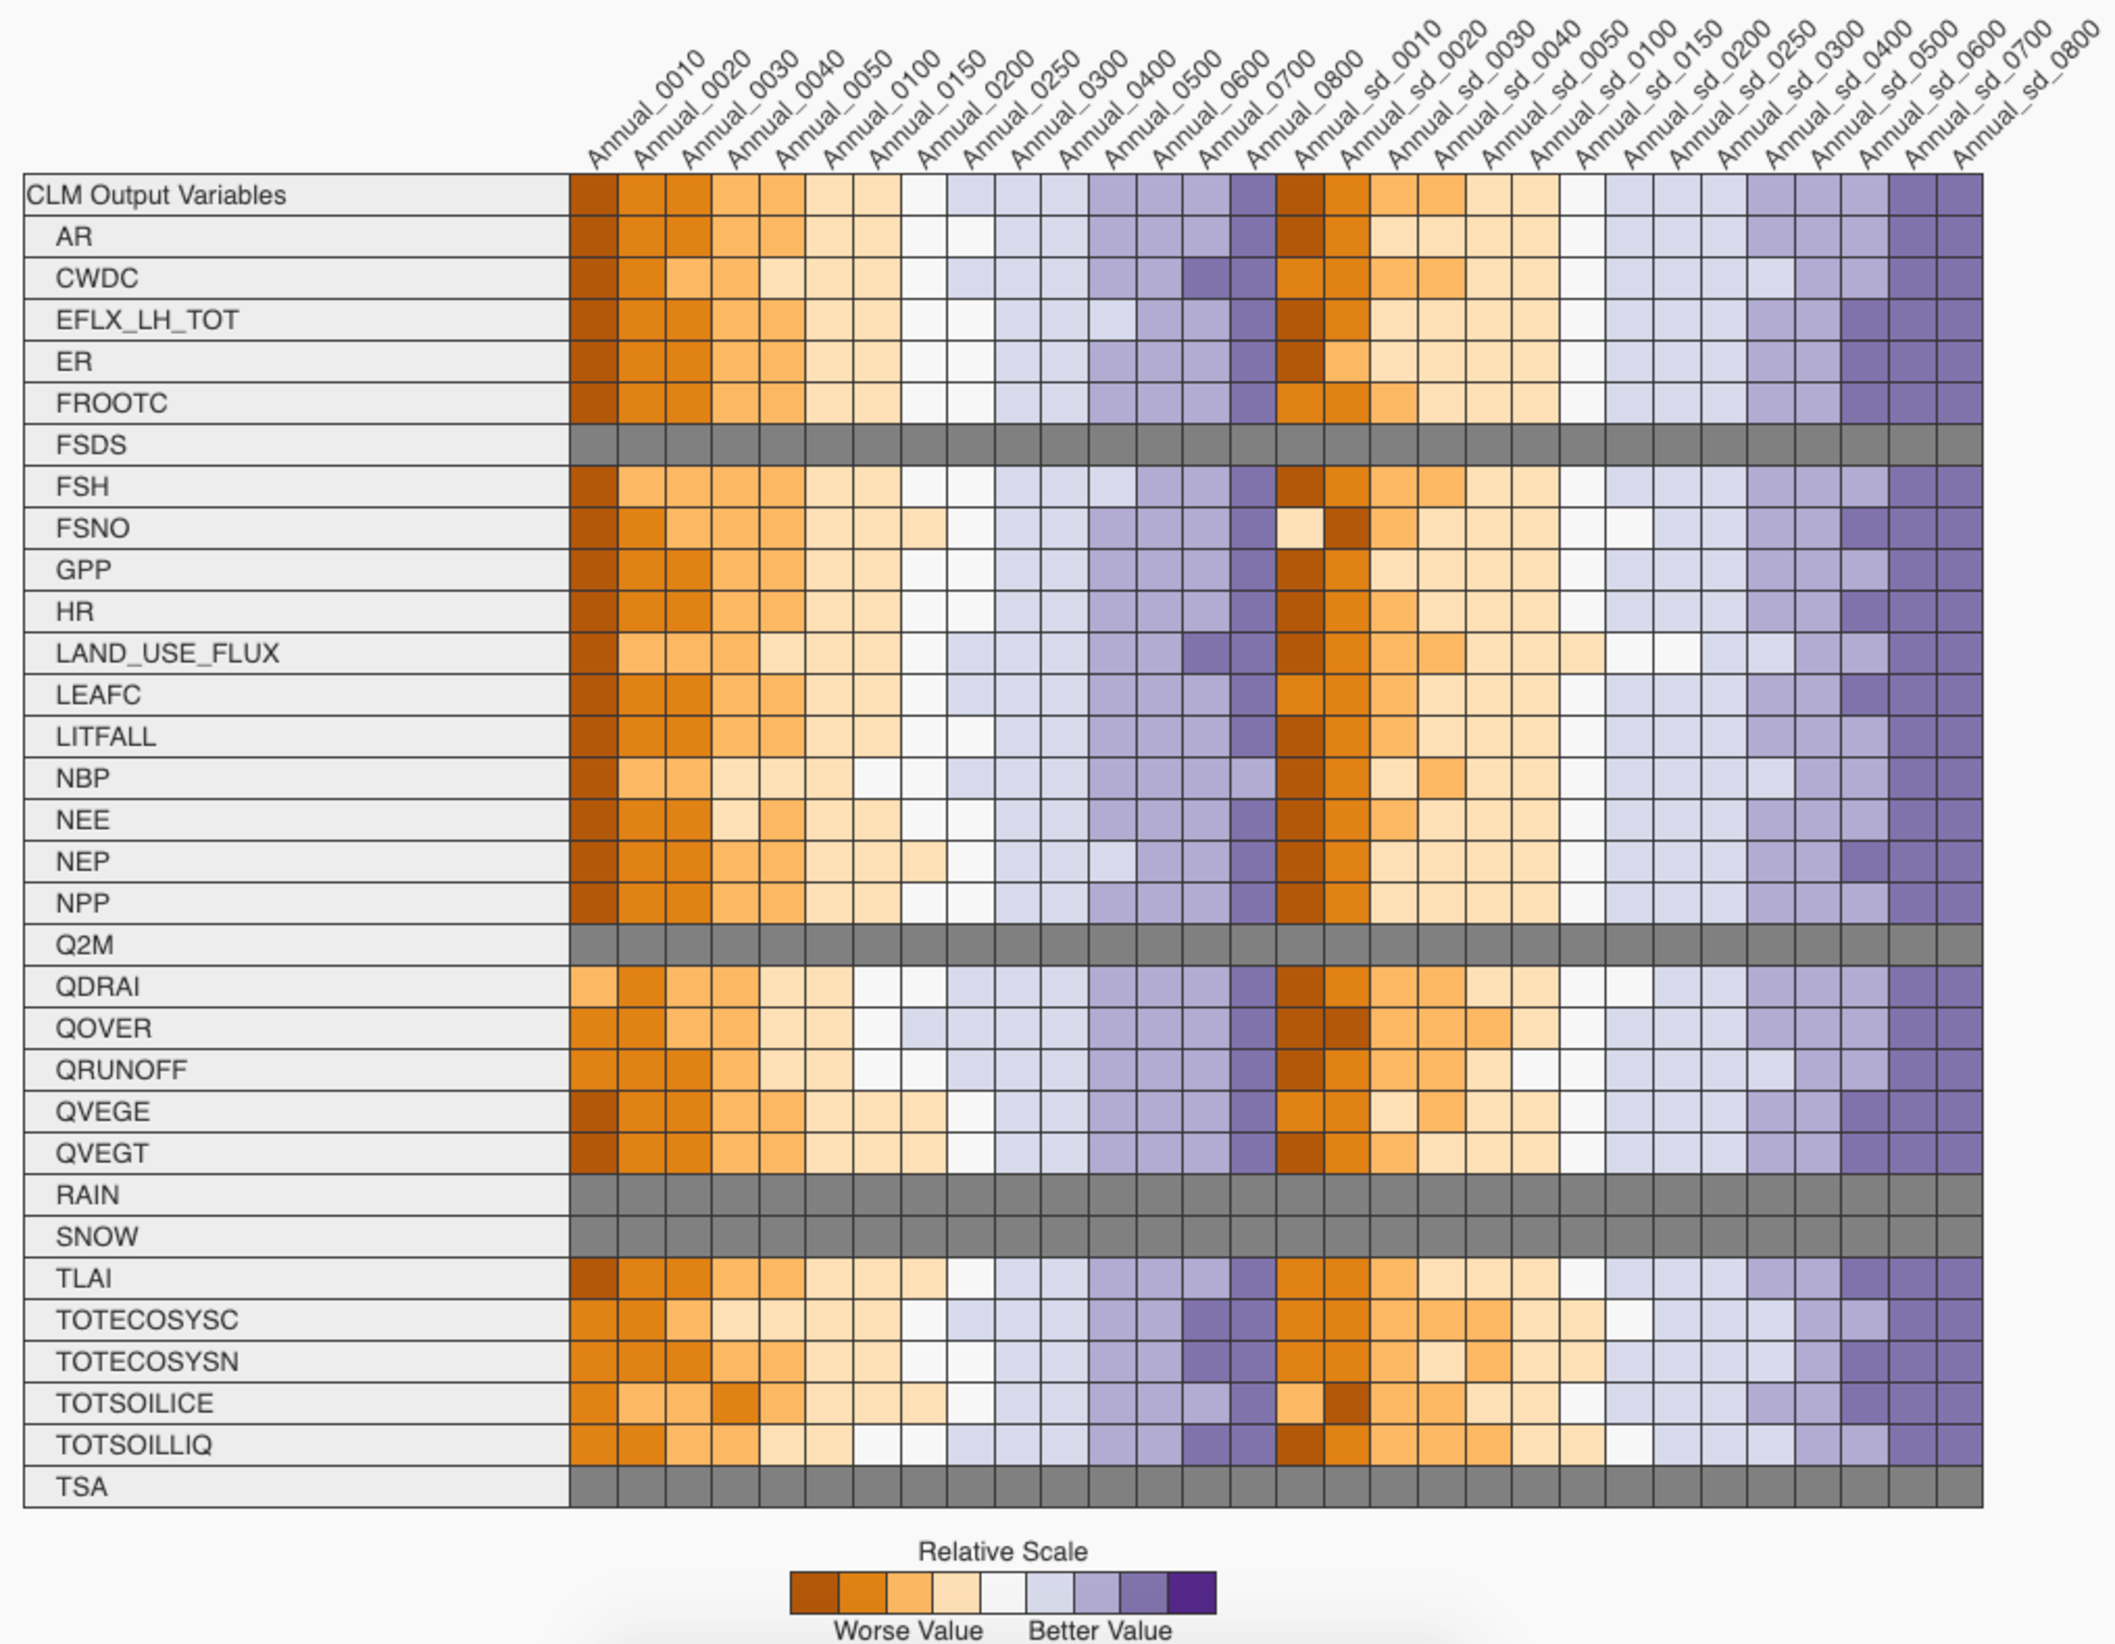
\includegraphics[width=42pc]{../figs/supp/ilamb.pdf}
\caption{ILAMB 2.5 overall scores comparing remapped sparsegrid output to the full grid 2$^{\circ}$ model output. Column headings indicate the number of clusters, and whether annual means or annual means and standard deviations were used as input to the clustering algorithm. We should try to remove the gray bits (zqz). Full, interactive results are available at \url{www.ilamb.org/PPE/CLM/2021-02}. See main text Section \ref{sect:sg} for clustering details.}
\label{supp:ilamb}
\end{figure}



\end{document}




